\subsection{Liczba bezpośrednich udostępnień }
Do tej analizy wzięto pod uwagę jedynie oryginalne posty, ponieważ mimo że na popularność tweeta ma znaczenie kto go udostępnił, bo to zapewnia większą grupę odbiorców, to popularność postu nie wpływa na statystykę popularności użytkowników, którzy dokonali dalszego udostępnienia. 
\par
Konta oznaczone jako factcheck publikują stosunkowo mało postów w\,porównaniu do innych klas. Jednak ich posty cieszą się dużą popularnością, jeśli chodzi o dalsze ich udostępnienie. Średnio post ma 18 retweetów, dzięki czemu 600 tweetów zostało powielone 11 tysięcy razy. Posty publikowane przez największe mainstremowe media nazywane tu Bigmainstream są średnio udostępniane przez 10 użytkowników. Ten wynik nie dziwi biorąc pod uwagę jak dużo osób obserwuje te konta.  
\par
Co ciekawe można zauważyć, że oryginalne posty mainstremowe w\,tym przedziale czasowym były udostępniane dalej przez średnio 2.9 użytkowników, czyli łącznie były udostępnione prawie 36 tysięcy razy. Średnia liczba retweetów posta opublikowanego przez Junk accounts wynosi 7.1 co oznacza ze te posty łącznie były udostępnione prawie 73\,tysięcy razy. Jest to dwa razy więcej niż łączna ilość udostępnień postów mainstreamowych mimo że postów mainstreamowych było 20 procent więcej oraz posiadają one łącznie trzy razy więcej followersów. 


\begin{table}[!h]
\centering
\caption{Porównanie liczby retweetów zebrancyh tweetów z podziałem na klasy.} \label{tab:liczbaretweetow}
\begin{tabular}{|m{2,8cm}|R{2,5cm}|R{2,5cm}|R{2,5cm}|}  
\hline
~Klasa & Liczba tweetów & Łączna liczba retweetów & Średnia liczba retweetów na tweet \\ 
\hline
NIERZETELNE & 10246 & 72975 & 7.1 \\ 
\hline
MAINSTREAM \textless{} 0,5 mln & 12566 & 35965 & 2.9 \\ 
\hline
MAINSTREAM \textgreater{} 0,5mln & 6463 & 61156 & 9.5 \\ 
\hline
FACTCHECK & 607 & 11020 & 18.2 \\
\hline
\end{tabular}
\end{table}



\subsubsection{Zróżnicowanie popularności kont}
Poniżej przedstawiono dwa wykresy omawiające w\,większych szczegółach charakterystykę udostępnień postów. Pierwszy z\,wykresów pokazuje średnią liczbę udostępnień oryginalnych postów dla najbardziej popularnych kont. Popularność konta oznacza tu liczbę udostępnień jakie otrzymują jego posty. Można też ją określić jako aktywność odbiorców. Jak widać na rysunku \ref{fig:retweets-per-tweet} popularność konta nie zależy od klasy do której należy i\,jest zróżnicowana w\,każdej klasie.
\begin{figure}[!h]
	\centering 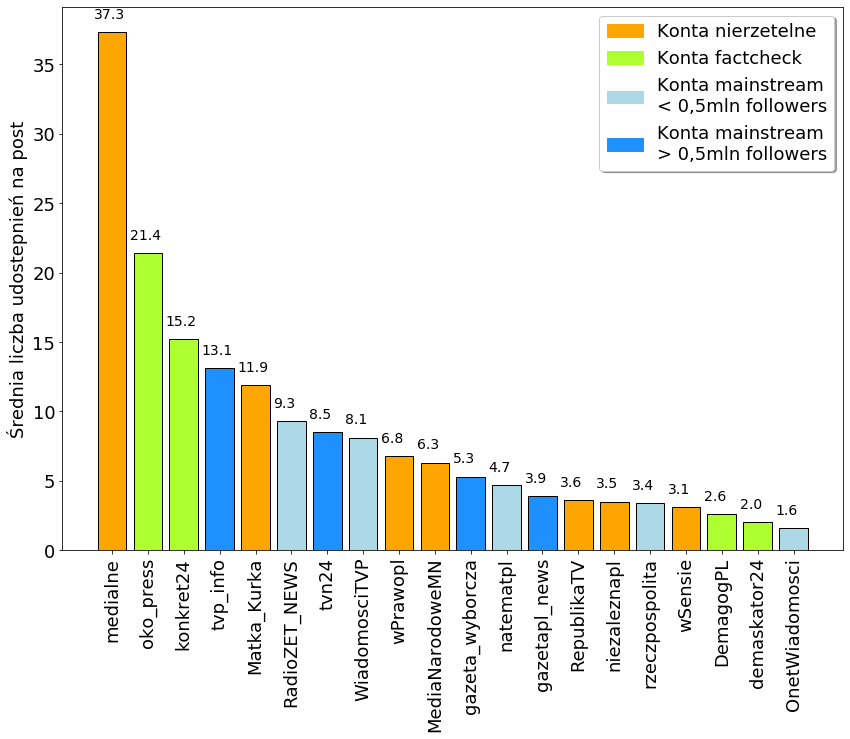
\includegraphics[width=0.95\linewidth]{img/results/retweetspertweet3.png}
	\caption{Wykres średniej liczby udostępnień oryginalnych tweetów dla najbardziej popularnych kont z\,podziałem na przynależność do klasy.} \label{fig:retweets-per-tweet}
\end{figure}

\subsubsection{Liczba followersów a\,popularność kont}
Następnie chciano zbadać czy na popularność treści publikowanych przez konta wpływa liczba jego subskrybentów. W\,tym celu stworzono wykres dwuwymiarowy w\,którym na osi x podano liczbę followers w\,skali logarytmicznej. Natomiast na osi y zaznaczono średnią liczbę udostępnień jaką otrzymują posty. Dodatkowo wielkością punktu na wykresie oznaczono aktywność konta liczoną jako średnia liczba postów publikowanych w\,czasie dnia. Wszystkie punkty zostały również oznaczone odpowiednim kolorem, w\,zależności, do której klasy należą. Zrezygnowano z\,nadania im nazw kont ze względu na czytelność wykresu, zwłaszcza, że w\,przypadku tego badania nie ma to większego znaczenia. 
\begin{figure}[!h]
	\centering 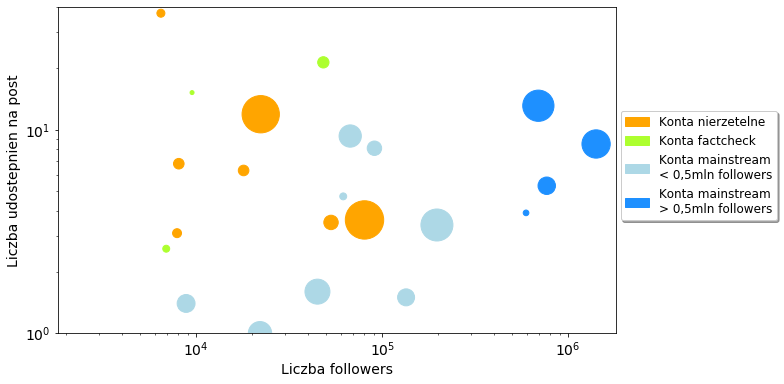
\includegraphics[width=0.95\linewidth]{img/results/retweetsvsfollowers2.png}
	\caption{Średnia liczba udostępnień tweeta a\,liczba followersów dla kont z\,podziałem na klasy.} \label{fig:retweets-vs-followers}
\end{figure}
\par

Na podstawie stworzonego wykresu można wyciągnąć wnioski, że ani liczba subskrybentów konta ani częstość publikacji nowych treści nie ma wyraźnie większego wpływu na aktywność odbiorców w\,liczbie udostępnień postów. Dwa konta o\,liczbie followersów większej niż pół miliona posiadają jedne z\,najwyższych popularności w\,tym zbiorze, jednak w\,tej klasyfikacji wyraźnie przewyższają je konta posiadające 10 razy mniejszą grupę odbiorców.  Podobnie nie widać żadnego schematu, aby odpowiednia liczba publikowanych postów w\,czasie dnia wpływała pozytywnie na aktywność odbiorców tych postów. 

